% Drawing 154/06-7 -- folder 154, batch 06, archive page 110 (PDF page 111).
% Transcription: en bas à gauche, quatre dessins en couleur de demi-cercles ou d'arcs vert clair aux extrémités marquées, avec des accolades au crayon portant des signes : « $-1$ » en haut et en bas, « $+1$ » sur les côtés et à l'intérieur dans le premier ; « $-1$ », « $+1$ » dans le deuxième ; dans les deux derniers, les côtés marqués « $\varepsilon$ » et l'intérieur « $+1$ », « $-1$ »
% Kind: four arcs with signed braces. Method 2 (schematic redraw from the facsimile). Status: ok.
% Notes: Bottom left of the (portrait) sheet, four drawings of light green half-circles or arcs with marked ends, with pencil braces carrying signs: « -1 » at the top and the bottom, « +1 » on the sides and inside in the first (which is closed by a light green base); « -1 », « +1 » in the second; in the last two, the sides marked « epsilon » and the inside « +1 », « -1 ». The braces are given by their signs only. Read from the page view.
% Coordinates: 1 unit = 1 mm = 1/100 of the crop width (bbox in page fractions: [0.144, 0.534, 0.535, 0.768]).
% Redrawn by Claude (claude-opus-5-5), issue #73, 2026-11-07; not checked by a human; not compiled (no TeX in the session).
% Revised by Claude (claude-opus-5-5) 2026-11-09 (issue #128) after Michel's check: vertices snapped to exact intersections (drawn points on their lines, meeting ends on the stroke they meet, near-concurrent lines through one computed point, curve ends on their rim); labels at \small as in folder 80 batch 3. Status: ok.
% Rights: reproduces part of the work -- behind RENDER_TRANSCRIPTS, never published by itself.
\documentclass[tikz,border=3pt]{standalone}
\usepackage{amsmath,amssymb}
\usetikzlibrary{patterns,arrows.meta}
\tikzset{Or/.style={orange!90!black}, Ye/.style={yellow!80!orange}, Lg/.style={green!60!black!70}, Dg/.style={green!45!black}, Br/.style={brown!80!black}, Rd/.style={red!85!black}, Bl/.style={blue!70!black}, Gy/.style={black!40}, pencil/.style={black!45}, struck/.style={black!35}, mark/.style={circle,draw,inner sep=1.3pt}, pt/.style={circle,fill,inner sep=0.9pt}, opt/.style={circle,draw,fill=white,inner sep=1.1pt}}
\colorlet{Or}{orange!90!black}\colorlet{Ye}{yellow!80!orange}\colorlet{Lg}{green!60!black!70}\colorlet{Dg}{green!45!black}\colorlet{Br}{brown!80!black}\colorlet{Rd}{red!85!black}\colorlet{Bl}{blue!70!black}\colorlet{Gy}{black!40}
\begin{document}
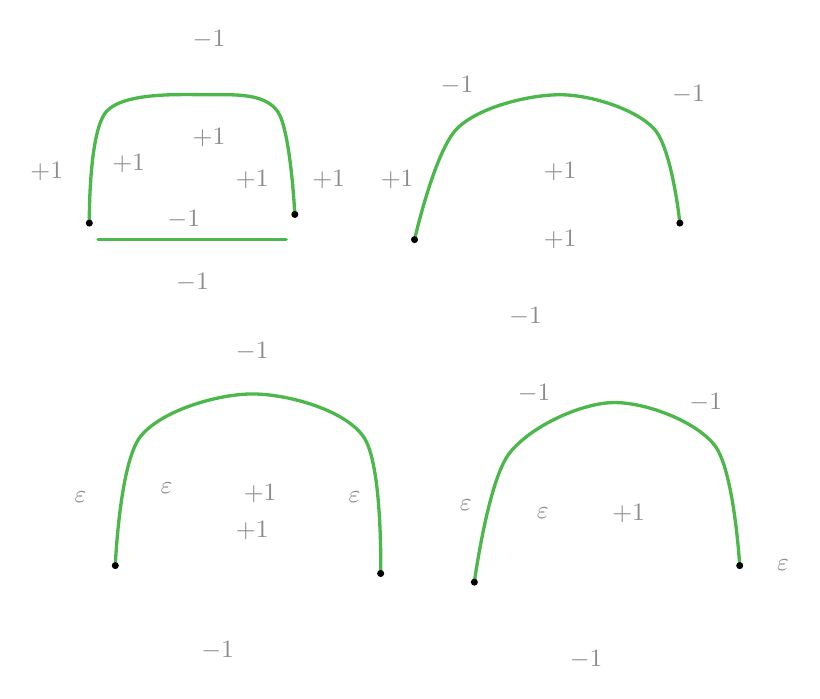
\begin{tikzpicture}[x=1mm,y=1mm,line cap=round,line join=round,font=\scriptsize]
\draw[Lg,very thick] plot[smooth, tension=0.55] coordinates {(7.6,-27.2) (9.8,-13) (22.8,-10.9) (31.5,-13) (33.7,-26.1)};
\node[pt] at (7.6,-27.2) {};
\node[pt] at (33.7,-26.1) {};
\draw[Lg,very thick] (8.7,-29.3) -- (32.6,-29.3);
\node[inner sep=1pt,pencil] at (22.8,-3.9) {\small $-1$};
\node[inner sep=1pt,pencil] at (20.7,-34.8) {\small $-1$};
\node[inner sep=1pt,pencil] at (2.2,-20.7) {\small $+1$};
\node[inner sep=1pt,pencil] at (38,-21.7) {\small $+1$};
\node[inner sep=1pt,pencil] at (12.6,-19.6) {\small $+1$};
\node[inner sep=1pt,pencil] at (22.8,-16.3) {\small $+1$};
\node[inner sep=1pt,pencil] at (28.3,-21.7) {\small $+1$};
\node[inner sep=1pt,pencil] at (19.6,-26.7) {\small $-1$};
\draw[Lg,very thick] plot[smooth, tension=0.55] coordinates {(48.9,-29.3) (54.3,-15.2) (67.4,-10.9) (79.3,-15.2) (82.6,-27.2)};
\node[pt] at (48.9,-29.3) {};
\node[pt] at (82.6,-27.2) {};
\node[inner sep=1pt,pencil] at (54.3,-9.8) {\small $-1$};
\node[inner sep=1pt,pencil] at (83.7,-10.9) {\small $-1$};
\node[inner sep=1pt,pencil] at (46.7,-21.7) {\small $+1$};
\node[inner sep=1pt,pencil] at (67.4,-20.7) {\small $+1$};
\node[inner sep=1pt,pencil] at (67.4,-29.3) {\small $+1$};
\node[inner sep=1pt,pencil] at (63,-39.1) {\small $-1$};
\draw[Lg,very thick] plot[smooth, tension=0.55] coordinates {(10.9,-70.7) (14.1,-54.3) (28.3,-48.9) (42.4,-54.3) (44.6,-71.7)};
\node[pt] at (10.9,-70.7) {};
\node[pt] at (44.6,-71.7) {};
\node[inner sep=1pt,pencil] at (28.3,-43.5) {\small $-1$};
\node[inner sep=1pt,pencil] at (6.5,-62) {\small $\varepsilon$};
\node[inner sep=1pt,pencil] at (17.4,-60.9) {\small $\varepsilon$};
\node[inner sep=1pt,pencil] at (41.3,-62) {\small $\varepsilon$};
\node[inner sep=1pt,pencil] at (29.3,-61.5) {\small $+1$};
\node[inner sep=1pt,pencil] at (28.3,-66.3) {\small $+1$};
\node[inner sep=1pt,pencil] at (23.9,-81.5) {\small $-1$};
\draw[Lg,very thick] plot[smooth, tension=0.55] coordinates {(56.5,-72.8) (60.9,-56.5) (73.9,-50) (87,-55.4) (90.2,-70.7)};
\node[pt] at (56.5,-72.8) {};
\node[pt] at (90.2,-70.7) {};
\node[inner sep=1pt,pencil] at (64.1,-48.9) {\small $-1$};
\node[inner sep=1pt,pencil] at (85.9,-50) {\small $-1$};
\node[inner sep=1pt,pencil] at (55.4,-63) {\small $\varepsilon$};
\node[inner sep=1pt,pencil] at (65.2,-64.1) {\small $\varepsilon$};
\node[inner sep=1pt,pencil] at (95.7,-70.7) {\small $\varepsilon$};
\node[inner sep=1pt,pencil] at (76.1,-64.1) {\small $+1$};
\node[inner sep=1pt,pencil] at (70.7,-82.6) {\small $-1$};
\end{tikzpicture}
\end{document}
